\begin{definition}[Grupo solúvel]
  Dezemos que $G$ é um \textbf{grupo solúvel} se existe uma sequencia finita $\{G_i\}_{i=1}^{n}$ de sugbrupos de $G$ taes que cumprem o papel de serem série abeliana, isso es
  \begin{align*}
    \{1\}=G_0\normal G_1\normal \cdots\normal G_n=G
  \end{align*}
  e $G_{i+1}/G_{i}$ é abelinao. 
\end{definition}
\begin{example}
  \begin{enumerate}
    \item Todo grupo abeliano é solúvel, ja que $\{1\}\normal G$.
    \item Se $G$ é simple, é solúvel, então $G$ é abeliano.
    \item $S_3$ é solúvel, poiss $\{1\}\normal \left\langle (123) \right\rangle\normal S_3$.
    \item $D_4$ é solúvel (\textcolor{red}{fazer diagrama}).
    \item $S_4$ é solúvel $\{1\}\normal K_4\normal A_4\normal S_4$.
    \item $S_n$ com $n\geq 5$ não é solúvel (vamos demonstrar isso mais tarde).
    \item $|G|=p^{3}$ é solúvel. Por um lado, se $G$ é abeliano, então $e$ solúvel. Por outro lado, se $G$ não é abeliano, então $|Z(G)|=p$, logo $\{1\}\normal Z(G)\normal G$.
    \item $|G|=p^{r}$, então $G$ é solúvel.\\
      Existe $H\leq G$ tal que $|H|=q$, logo $[G:H]=p$, logo $H\normal G$ (porque é abeliano). Assim, $\{1\}\normal H\normal G$. 
  \end{enumerate}
\end{example}
\begin{theorem}[Teorema de Burniside]
  Se $G$ é um grupo tal que $|G|=p^{a}q^{b}$, então $G$ é solúvel. 
\end{theorem}
\begin{proposition}[Propriedades do um grupo solúvel]
  \begin{enumerate}
    \item Se $H\leq G$, então $H$ é solúvel.
    \item Se $N\normal G$, então $G/N$ é solúvel.
    \item Se $N\normal G$, $N$ solúvel e $G/N$ é solúvel, então $G$ é solúvel. 
  \end{enumerate}
\end{proposition}
\begin{proof} 
  \begin{enumerate}
    \item Vamos seguir o diagrama abaixo.\\
      \begin{center}
        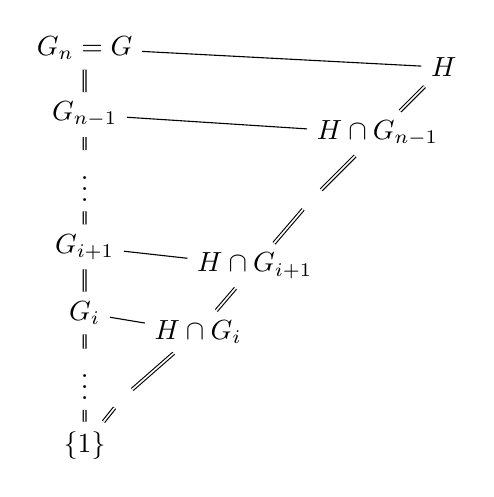
\begin{tikzpicture}[scale=1.2]
  % Nodes
  \node (Gn) at (-1,2.1) {$G_n=G$};
  \node (Gn-1) at (-1,1.4) {$G_{n-1}$};
  \node (p1) at (-1,0.7) {$\vdots$};
  \node (Gi+1) at (-1,0) {$G_{i+1}$};
  \node (Gi) at (-1,-0.7) {$G_i$};
  \node (p2) at (-1,-1.4) {$\vdots$};
  \node (1) at (-1,-2.1) {$\{1\}$};
  \node (H) at (2.8,1.9) {$H$};
  \node (HGn-1) at (2.1,1.2) {$H\cap G_{n-1}$};
  \node (p3) at (1.4,0.5) {$\iddots$};
  \node (HGi+1) at (0.8,-0.2) {$H\cap G_{i+1}$};
  \node (HGi) at (0.2,-0.9) {$H\cap G_i$};
  \node (p4) at (-0.6,-1.6) {$\iddots$};

  % Lineas nodos
  \draw[double] (Gn) -- (Gn-1);
  \draw[double] (Gn-1) -- (p1);
  \draw[double] (p1) -- (Gi+1);
  \draw[double] (Gi+1) -- (Gi);
  \draw[double] (Gi) -- (p2);
  \draw[double] (p2) -- (1);
  \draw (Gn) -- (H);
  \draw (Gn-1) -- (HGn-1);
  \draw (Gi+1) -- (HGi+1);
  \draw (Gi) -- (HGi);
  \draw[double] (H) -- (HGn-1);
  \draw[double] (HGn-1) -- (p3);
  \draw[double] (p3) -- (HGi+1);
  \draw[double] (HGi+1) -- (HGi);
  \draw[double] (HGi) -- (p4);
  \draw[double] (p4) -- (1);
\end{tikzpicture}
  
      \end{center}
      \begin{itemize}
        \item Defina $H_i=H\cap G_i$. Logo $H_i\normal H_i+1$.
        \item Temos que
          \begin{align*}
            H_{i+1}/H_{i}&=\frac{H\cap G_{i+1}}{H\cap G_i}\\
            &=\frac{H\cap G_{i+1}}{(H\cap G_{i+1})\cap G_{i}}\\
            &\cong \frac{(H\cap G_{i+1})G_{i}}{G_i} \leq G_{i+1}/G_{i}, \text{ é abeliano}.
          \end{align*}
      \end{itemize}
      Logo $H$ é solúvel.
    \item Vamos segui o diagrama abaixo.\\
      \begin{center}  
        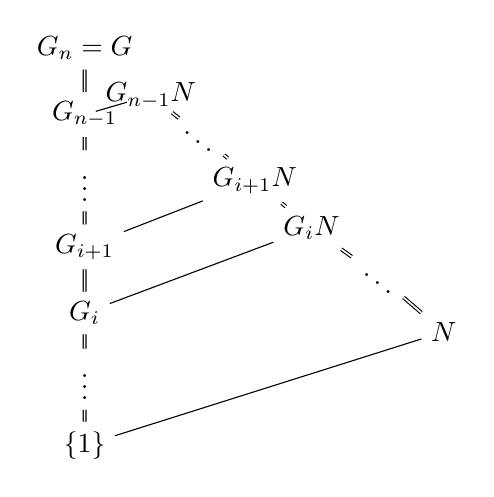
\begin{tikzpicture}[scale=1.2]
  % Nodes
  \node (Gn) at (-1,2.1) {$G_n=G$};
  \node (Gn-1) at (-1,1.4) {$G_{n-1}$};
  \node (p1) at (-1,0.7) {$\vdots$};
  \node (Gi+1) at (-1,0) {$G_{i+1}$};
  \node (Gi) at (-1,-0.7) {$G_i$};
  \node (p2) at (-1,-1.4) {$\vdots$};
  \node (1) at (-1,-2.1) {$\{1\}$};
  \node (Gn-1N) at (-0.3,1.6) {$G_{n-1}N$};
  \node (p3) at (0.2,1.2) {$\ddots $};
  \node (Gi+1N) at (0.8,0.7) {$G_{i+1}N$};
  \node (GiN) at (1.4,0.2) {$G_iN$};
  \node (p4) at (2.1,-0.3) {$\ddots$};
  \node (N) at (2.8,-0.9) {$N$};

  % Lineas nodos
  \draw[double] (Gn) -- (Gn-1);
  \draw[double] (Gn-1) -- (p1);
  \draw[double] (p1) -- (Gi+1);
  \draw[double] (Gi+1) -- (Gi);
  \draw[double] (Gi) -- (p2);
  \draw[double] (p2) -- (1);
  \draw (Gn-1) -- (Gn-1N);
  \draw (Gi+1) -- (Gi+1N);
  \draw (Gi) -- (GiN);
  \draw (1) -- (N);
  \draw[double] (Gn-1N) -- (p3);
  \draw[double] (p3) -- (Gi+1N);
  \draw[double] (Gi+1N) -- (GiN);
  \draw[double] (GiN) -- (p4);
  \draw[double] (p4) -- (N);
\end{tikzpicture}
  
      \end{center}
      \begin{itemize}
        \item Seja $\{G_kN/N\}$ a sequencia.
        \item $G_iN/N\normal G_{i+1}N/N$.
        \item $\frac{G_{i+1}N/N}{G_iN/N}$ é abeliano. 
      \end{itemize}
    \item Como $G/N=\overline{G}$  é solúvel, existe seguinte $\{\overline{G}_i\}$ tal que
      $$\{\overline{1}\}=\overline{G}_0\normal \overline{G}_1\normal \cdots\normal \overline{G}_n=G/N.$$
      Pelo teorema de correspondencia temos que existen $G_i$ tales que
      $$N\normal G_1\normal \cdots\normal G_{n-1}\normal G_n.$$
      E como $N$ é solúvel
      $$\{1\}\normal \overline{G}_1\normal\cdots\normal N\normal G_1\normal \cdots\normal G_{n-1}\normal G_n.$$
  \end{enumerate}
\end{proof}
\begin{definition}[Série derivada]
  Seja $G$ um grupo. Se definimos $G^{(0)}=G,G^{(1)}=G^{\prime},G^{(i+1)}=(G^{(i)})^{\prime}$, então chamamos $\{G^{(i)}\}_{i\geq 0}$ \text{série derivada} de $G$. 
\end{definition}
\begin{proposition}
  $G$ é soluvél se, somente se, existe $m\in\mathbb{N}$ tal que $G^{(m)}=\{1\}$. 
\end{proposition}
